\documentclass[11pt]{article}
\usepackage{charter}
\usepackage{graphicx}
\usepackage{hyperref}
\usepackage[margin=1in]{geometry}
\usepackage{amsmath}

\hypersetup{
	colorlinks=true,
	linkcolor=blue,
	filecolor=magenta,
	urlcolor=cyan,
}

\begin{document}

%===================================================
% Title and Author Info
%===================================================
\begin{center}
{\Large\textsc{Stable Keplerian Orbits}} \\
\vspace{10pt}
{\large \textbf{Mentor:} Alex Urban} \\
{\small LIGO Laboratory, California Institute of Technology \\
Pasadena, CA 91125, USA \\
\href{mailto:aurban@ligo.caltech.edu}{\texttt{aurban@ligo.caltech.edu}}}
\end{center}

\section*{Purpose}

\hspace{15pt} In this problem, we will work out the total energy of a stable Keplerian orbit and simulate it in Python. The goal is, once again, to use what we understand now to inform what we're going to do next: with a growing intuition for the astrophysics of compact binaries, we will now implement an awesome Keplerian orbit simulation.... \textit{of science!}

\section*{Stable Keplerian Orbits}
\hspace{15pt} Suppose that a neutron star binary (each with mass $M = 1.4\,\, M_{\odot}$) is in a stable, Keplerian orbit (\textit{i.e.} with no loss of energy). Figure \ref{fig:binary_diagram} illustrates this system.

\begin{enumerate}

\item Using Kepler's laws, show that when the orbit is perfectly circular, the azimuthal angle $\varphi$ is a linear function of time. (You can presume the orbit is in a plane, so $\theta = \pi/2 =$ const.)

\item Write the angular velocity $\omega = d\varphi/dt$ in terms of $a$ and the orbital angular momentum, $L$, and plot $L$ and $v=a\omega$ \textit{vs.} the gravitational wave frequency for circular orbits. (Remember that the LIGO instruments are sensitive to binary neutron stars up to about 3000 or 4000 Hz, so that should be the range of your plot.)

\item Show that if $a$ is allowed to vary (still with no energy loss!), then the total energy is
\begin{equation}
E = \frac{M}{4}\left(\frac{da}{dt}\right)^2 + \Phi(a; L)
\end{equation}
where the function
\begin{equation}
\Phi(a; L) = - \frac{GM^2}{a} + \frac{L^2}{Ma^2}
\end{equation}
is called the \textit{effective potential}. (Note that $L$ is conserved during a Keplerian orbit, so the effective potential only depends on $a$.)

\item Find the critical points of $\Phi$ with respect to $a$, and plot the effective potential for $2L^2/GM^3 =$ 0, 20, 40, and 60 km. What physics do these critical points tell us? How can we interpret the term in $\Phi$ that depends on $L^2$?

\item Try writing a Python simulation using \href{https://en.wikipedia.org/wiki/Euler_method}{Euler's method} to integrate the equations for $a$ and $\varphi$ using arbitrary values for $E$, $L$, and the initial velocity. As a sanity check, your simulation should plot the total energy and orbital angular momentum (both should be constant), along with $a$, $\varphi$, and the orbital velocity, all as a function of time. The simulation should also draw complete orbits in polar coordinates, experimenting with different initial conditions.

\item Now, combine these results with last week's. What energies and angular momenta give us stable circular orbits in the region where 30 Hz $\leq f_{\rm GW} \leq$ 3000 Hz? What does the centrifugal force on each neutron star look like in this region? How does this compare with the tidal force?

\end{enumerate}

\vspace{30pt}

\begin{figure}[!h]
\centering
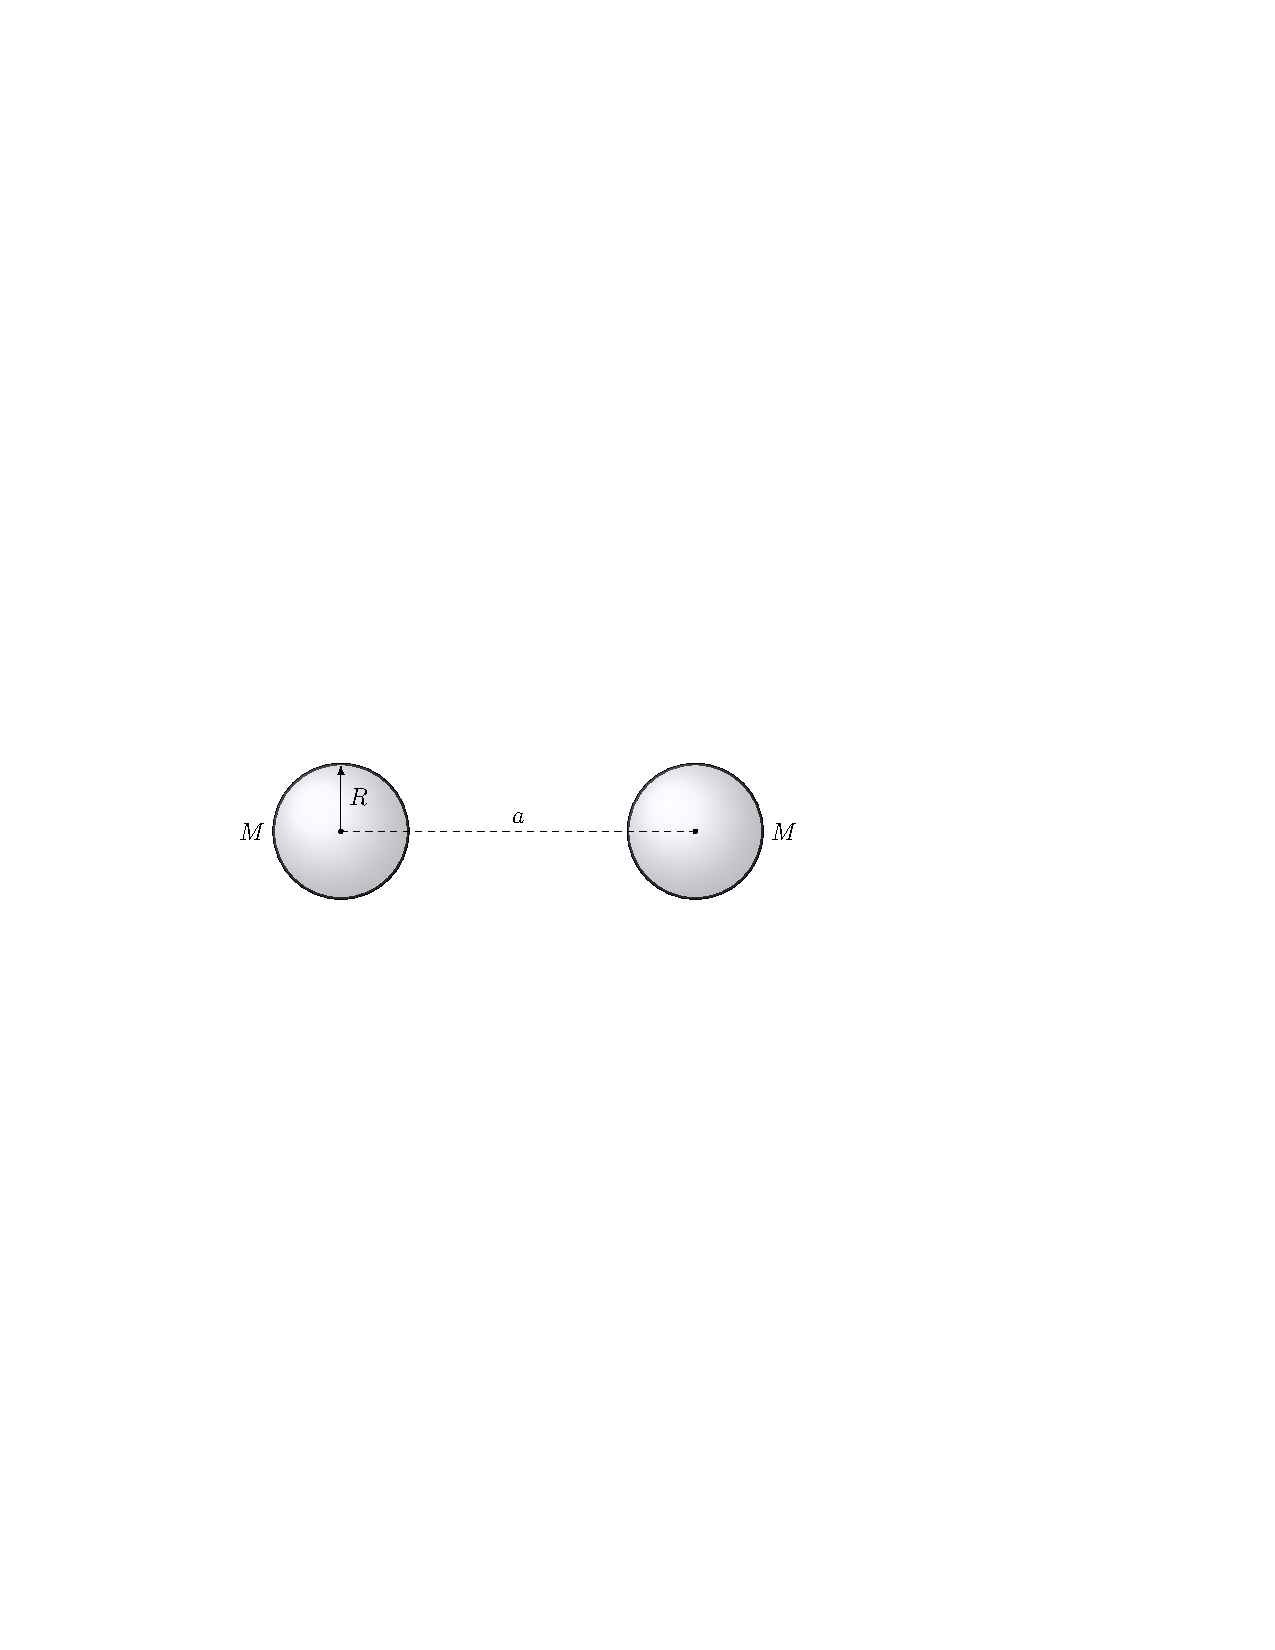
\includegraphics{binary_diagram.pdf}
\caption{\label{fig:binary_diagram}Diagram of the neutron star binary, showing its orbital separation ($a$) and the radius ($R$) and masses ($M$) of the individual neutron stars. The various mutual gravitational forces at play are also illustrated.}
\end{figure}

\end{document}
